\documentclass[a4paper,12pt]{article}
\usepackage{amsmath}
\usepackage[utf8x]{inputenc}
%\usepackage{amstext}
\usepackage{graphicx}
\usepackage{color}
\usepackage[left=2cm, top=2cm, right=3cm,
bottom=2cm]{geometry}
%\usepackage[landscape]{geometry}
%\usepackage{lscape}
\usepackage{pdfpages}

\author{Katja Matilainen \\ University of Oulu}
\title{Stellar structure and evolution \\ Computer assignment for advanced students}
\date{Spring 2015}

\begin{document}

\begin{tiny}
\maketitle
\end{tiny}

\vspace{0.5cm}
\begin{itemize}

\item[\textbf{Part 1.}]

Solve the Lane-Emden equation for $n=0$, $n=0.5$, $n=1$, $n=1.5$, $n=2$, $n=2.5$, $n=3$, $n=3.5$, $n=4$, $n=4.5$, and $n=5$. Plot the results.

\vspace{0.5cm}
\textbf{Solution}

The function for solving the Lane-Emden equation for given $n$:

\begin{scriptsize}
\begin{verbatim}
;------------------------------------------------------------------------;
; lane_emden.pro
;------------------------------------------------------------------------;
; Description:
; Function for solving the Lane-Emden equation for given polytropic
; index n. Creates vector ksi and solves theta for those values.
; Also added: return dTheta/dKsi

; Input: n
; Output: array result=[[ksi], [theta],[dtheta_dksi]]
;------------------------------------------------------------------------;

function lane_emden,n
;------------------------------------------------------------------------;
; Polytropic index
;------------------------------------------------------------------------;
; Polytropic index n is taken from the input
n=n

;------------------------------------------------------------------------;
; Vector ksi
;------------------------------------------------------------------------;
; Ksi has values in the range [0,100]
ksi=findgen(100000)*0.001d0

; Vectors dTheta/dKsi and Theta have the same amount of components as Ksi
dtheta_dksi=ksi*0.d0
theta=ksi*0.d0

;------------------------------------------------------------------------;
; Lane-Emden equation
;------------------------------------------------------------------------;
;Loop that solves theta[i] from ksi[i]

;Starting values
i=1
dtheta_dksi[0]=0.d0
ksi[0]=0.d0
theta[0]=1.d0

;Integration loop
while theta[i-1] gt 0.d0 do begin
if i ge n_elements(ksi) then break
;Theta
   theta[i]=theta[i-1]+(ksi[i]-ksi[i-1])*dtheta_dksi[i-1]
;Derivative of theta
   dtheta_dksi[i]=dtheta_dksi[i-1]-(ksi[i]-ksi[i-1])*(theta[i-1]^n+2.d0/ksi[i]*dtheta_dksi[i-1])
;Increase index i
   i=i+1
endwhile

;------------------------------------------------------------------------;
;Cut the zeroes away from the end of the theta -vector, and
;make ksi to be the same lenght as theta.
;------------------------------------------------------------------------;

;Make new vectors ksi0 and theta0
ksi0=0.d0
theta0=1.d0
dtheta_dksi0=0.d0

j=1
while theta[j-1] gt 0.d0 do begin
if j ge n_elements(ksi) then break
theta0=[theta0,theta[j]]
ksi0=[ksi0,ksi[j]]
dtheta_dksi0=[dtheta_dksi0,dtheta_dksi[j]]
j=j+1
endwhile

;Result array is [[ksi0],[theta0],[dtheta_dksi0]]
result=[[ksi0],[theta0],[dtheta_dksi0]]

return,result
end
\end{verbatim}
\end{scriptsize}

The main program, that calls the previously defined function for solving the Lane-Emden equation, and plots the results as $( \xi , \theta)$ for all requested values of $n$:

\begin{scriptsize}
\begin{verbatim}
;------------------------------------------------------------------------;
; Stellar structure and evolution
; Computer assignment for advanced students
;------------------------------------------------------------------------;
;  PART I
;------------------------------------------------------------------------;
; Use the subroutine PsPlot to save results in a postscript plot 
; (written by Heikki Salo)
;------------------------------------------------------------------------;

pro PsPlot,routine,filename
	thisdir=getenv('PWD')+'/'
	psopen,/color,dir=thisdir,filename
	call_procedure,routine
	psclose		
end
;------------------------------------------------------------------------;

;------------------------------------------------------------------------;
;  MAIN PROGRAM starts here
;------------------------------------------------------------------------;
; Solve the Lane-Emden equation for
; n=[0,0.5,1,1.5,2,2.5,3,3.5,4,4.5,5]
; and plot the results (ksi,theta).

pro stellar_part1

;Use the function lane_emden for solving the Lane-Emden equation

;------------------------------------------------------------------------;
;For n=0
;------------------------------------------------------------------------;
n1=0
results1=lane_emden(n1)
;Separate the results
ksi1=results1[*,0]
theta1=results1[*,1]

;Plot the results as (ksi,theta) for all values of n
plot,ksi1,theta1,xrange=[0,10],yrange=[-0.1,1.1],title='Lane-Emden',xtitle='!9x!X!N',ytitle='!9q!X!N'
oplot,[0,10],[0,0],linestyle=1
xyouts,2.1,-0.05,'n=0'

;------------------------------------------------------------------------;
;For n=0.5
;------------------------------------------------------------------------;
n2=0.5
results2=lane_emden(n2)
;Separate the results
ksi2=results2[*,0]
theta2=results2[*,1]

;Plot the results as (ksi,theta) for all values of n
oplot,ksi2,theta2
xyouts,2.5,-0.05,'n=0.5'

;------------------------------------------------------------------------;
;For n=1
;------------------------------------------------------------------------;
n3=1
results3=lane_emden(n3)
;Separate the results
ksi3=results3[*,0]
theta3=results3[*,1]

;Plot the results as (ksi,theta) for all values of n
oplot,ksi3,theta3
xyouts,3.1,-0.05,'n=1'

;------------------------------------------------------------------------;
;For n=1.5
;------------------------------------------------------------------------;
n4=1.5
results4=lane_emden(n4)
;Separate the results
ksi4=results4[*,0]
theta4=results4[*,1]

;Plot the results as (ksi,theta) for all values of n
oplot,ksi4,theta4
xyouts,3.55,-0.05,'n=1.5'

;------------------------------------------------------------------------;
;For n=2
;------------------------------------------------------------------------;
n5=2
results5=lane_emden(n5)
;Separate the results
ksi5=results5[*,0]
theta5=results5[*,1]

;Plot the results as (ksi,theta) for all values of n
oplot,ksi5,theta5
xyouts,4.25,-0.05,'n=2'

;------------------------------------------------------------------------;
;For n=2.5
;------------------------------------------------------------------------;
n6=2.5
results6=lane_emden(n6)
;Separate the results
ksi6=results6[*,0]
theta6=results6[*,1]

;Plot the results as (ksi,theta) for all values of n
oplot,ksi6,theta6
xyouts,5.25,-0.05,'n=2.5'

;------------------------------------------------------------------------;
;For n=3
;------------------------------------------------------------------------;
n7=3
results7=lane_emden(n7)
;Separate the results
ksi7=results7[*,0]
theta7=results7[*,1]

;Plot the results as (ksi,theta) for all values of n
oplot,ksi7,theta7
xyouts,6.75,-0.05,'n=3'

;------------------------------------------------------------------------;
;For n=3.5
;------------------------------------------------------------------------;
n8=3.5
results8=lane_emden(n8)
;Separate the results
ksi8=results8[*,0]
theta8=results8[*,1]

;Plot the results as (ksi,theta) for all values of n
oplot,ksi8,theta8
xyouts,9.2,-0.05,'n=3.5'

;------------------------------------------------------------------------;
;For n=4
;------------------------------------------------------------------------;
n9=4
results9=lane_emden(n9)
;Separate the results
ksi9=results9[*,0]
theta9=results9[*,1]

;Plot the results as (ksi,theta) for all values of n
oplot,ksi9,theta9
xyouts,9.4,0.08,'n=4'

;------------------------------------------------------------------------;
;For n=4.5
;------------------------------------------------------------------------;
n10=4.5
results10=lane_emden(n10)
;Separate the results
ksi10=results10[*,0]
theta10=results10[*,1]

;Plot the results as (ksi,theta) for all values of n
oplot,ksi10,theta10
xyouts,9,0.145,'n=4.5'

;------------------------------------------------------------------------;
;For n=5
;------------------------------------------------------------------------;
n11=5
results11=lane_emden(n11)
;Separate the results
ksi11=results11[*,0]
theta11=results11[*,1]

;Plot the results as (ksi,theta) for all values of n
oplot,ksi11,theta11
xyouts,8.6,0.21,'n=5'

end

;--------------------------------------------------------------------;
; Save the results to a PostScript file using PsPlot
;--------------------------------------------------------------------;

pro Plot_everything
PsPlot, 'stellar_part1', 'stellar_part1.ps'
end

\end{verbatim}
\end{scriptsize}

\newpage
\vspace{0.5cm}
\textbf{Results}
\vspace{0.5cm}

The final results as $( \xi , \theta)$ for all requested values of $n$.

\centerline{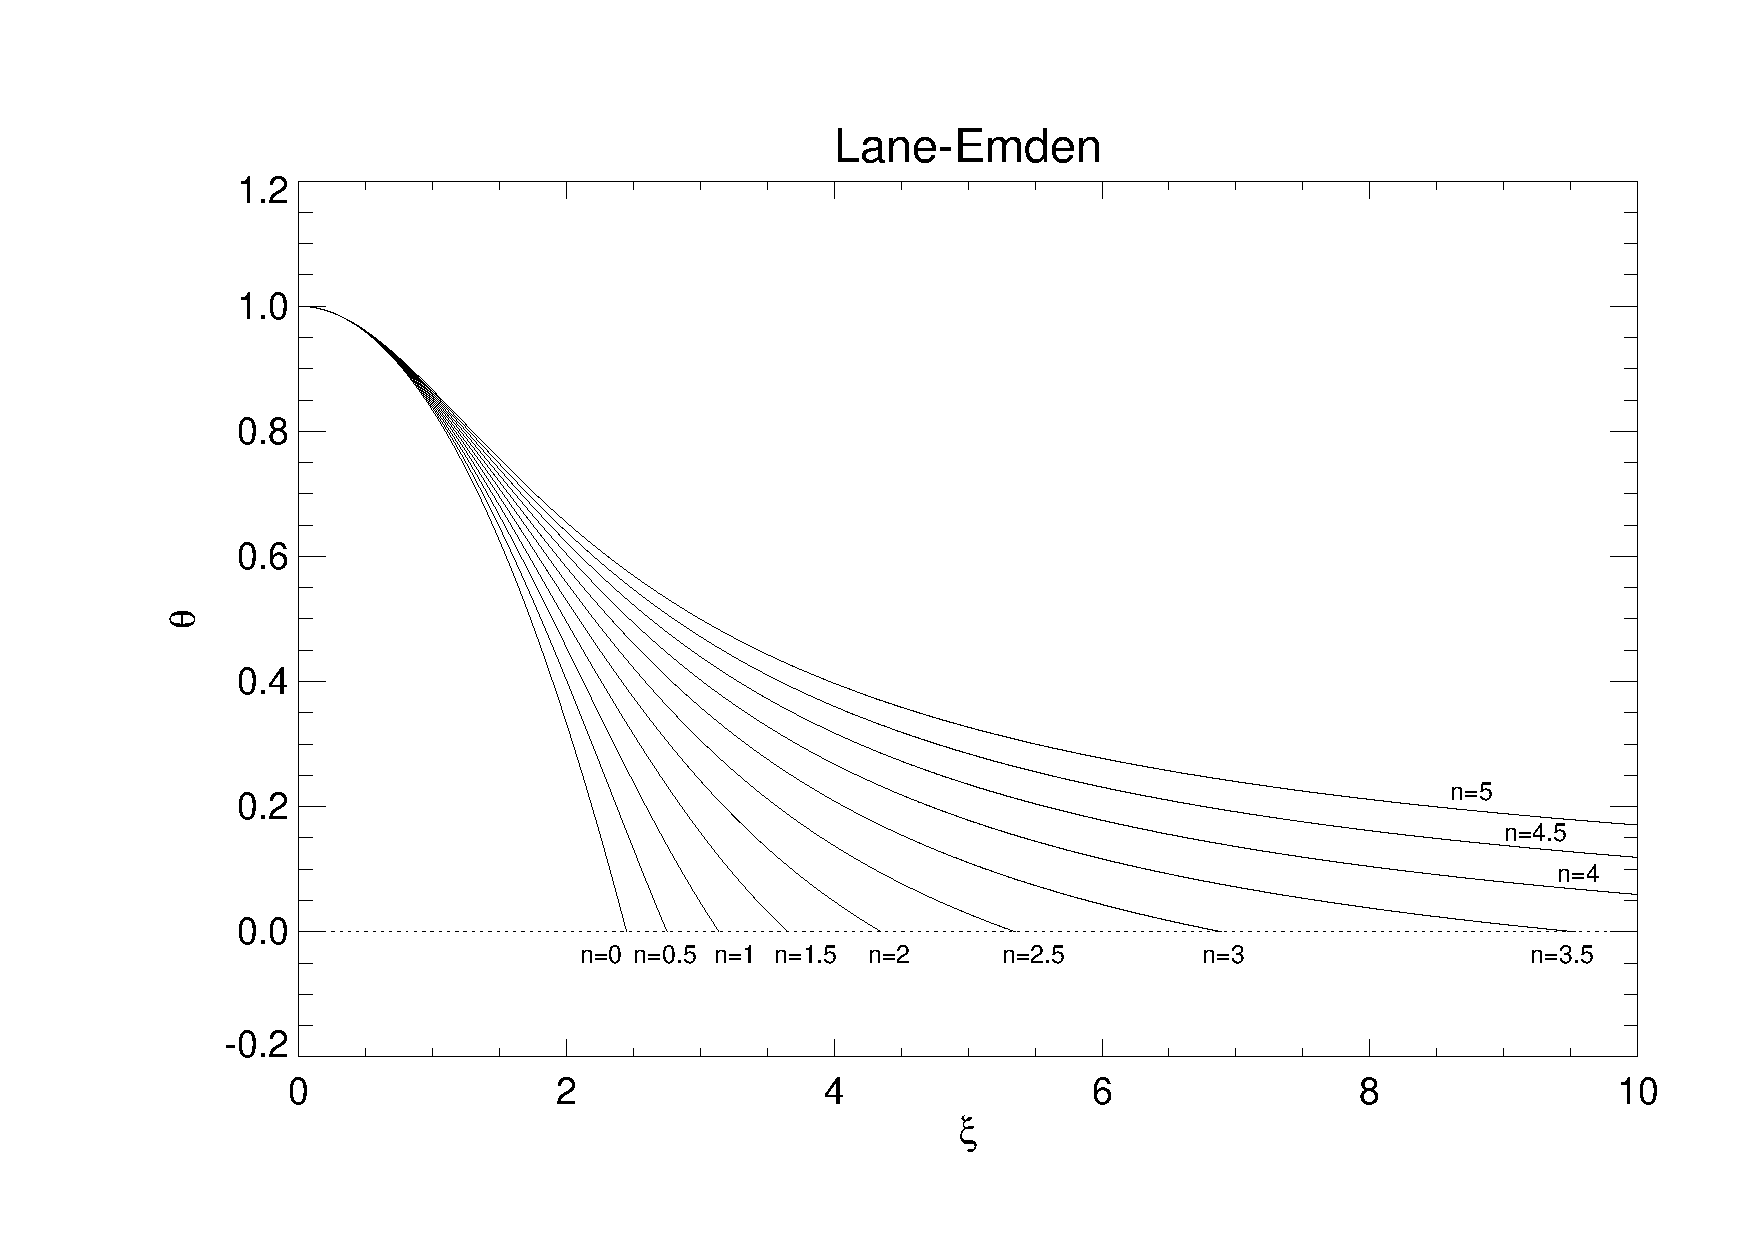
\includegraphics[scale=0.7]{stellar_part1.pdf}}

\newpage
\item[\textbf{Part 2.}]

In the two cases where we have found analytical solutions to the Lane-Emden equation, compare them to your numerical derivations, so you can check that everything is correct.

\vspace{0.5cm}
\textbf{Answer:}

In the exercises we solved the Lane-Emden equation analytically for $n=0$ and $n=1$.

For $n=0$ the solution was 

\begin{equation}
\theta(\xi)=-\frac{1}{6}\xi^2+1 \, ,
\end{equation}

which is a downwards opening parabola that crosses the $\theta$ axis at $\theta=1$ and the $\xi$ axis at $\xi_1=\sqrt{6} \approx 2.44949 $.
%When plotted in IDL the analytical solution looks like:

In IDL the numerical (black line) and analytical (grey line) solutions look like this:

\centerline{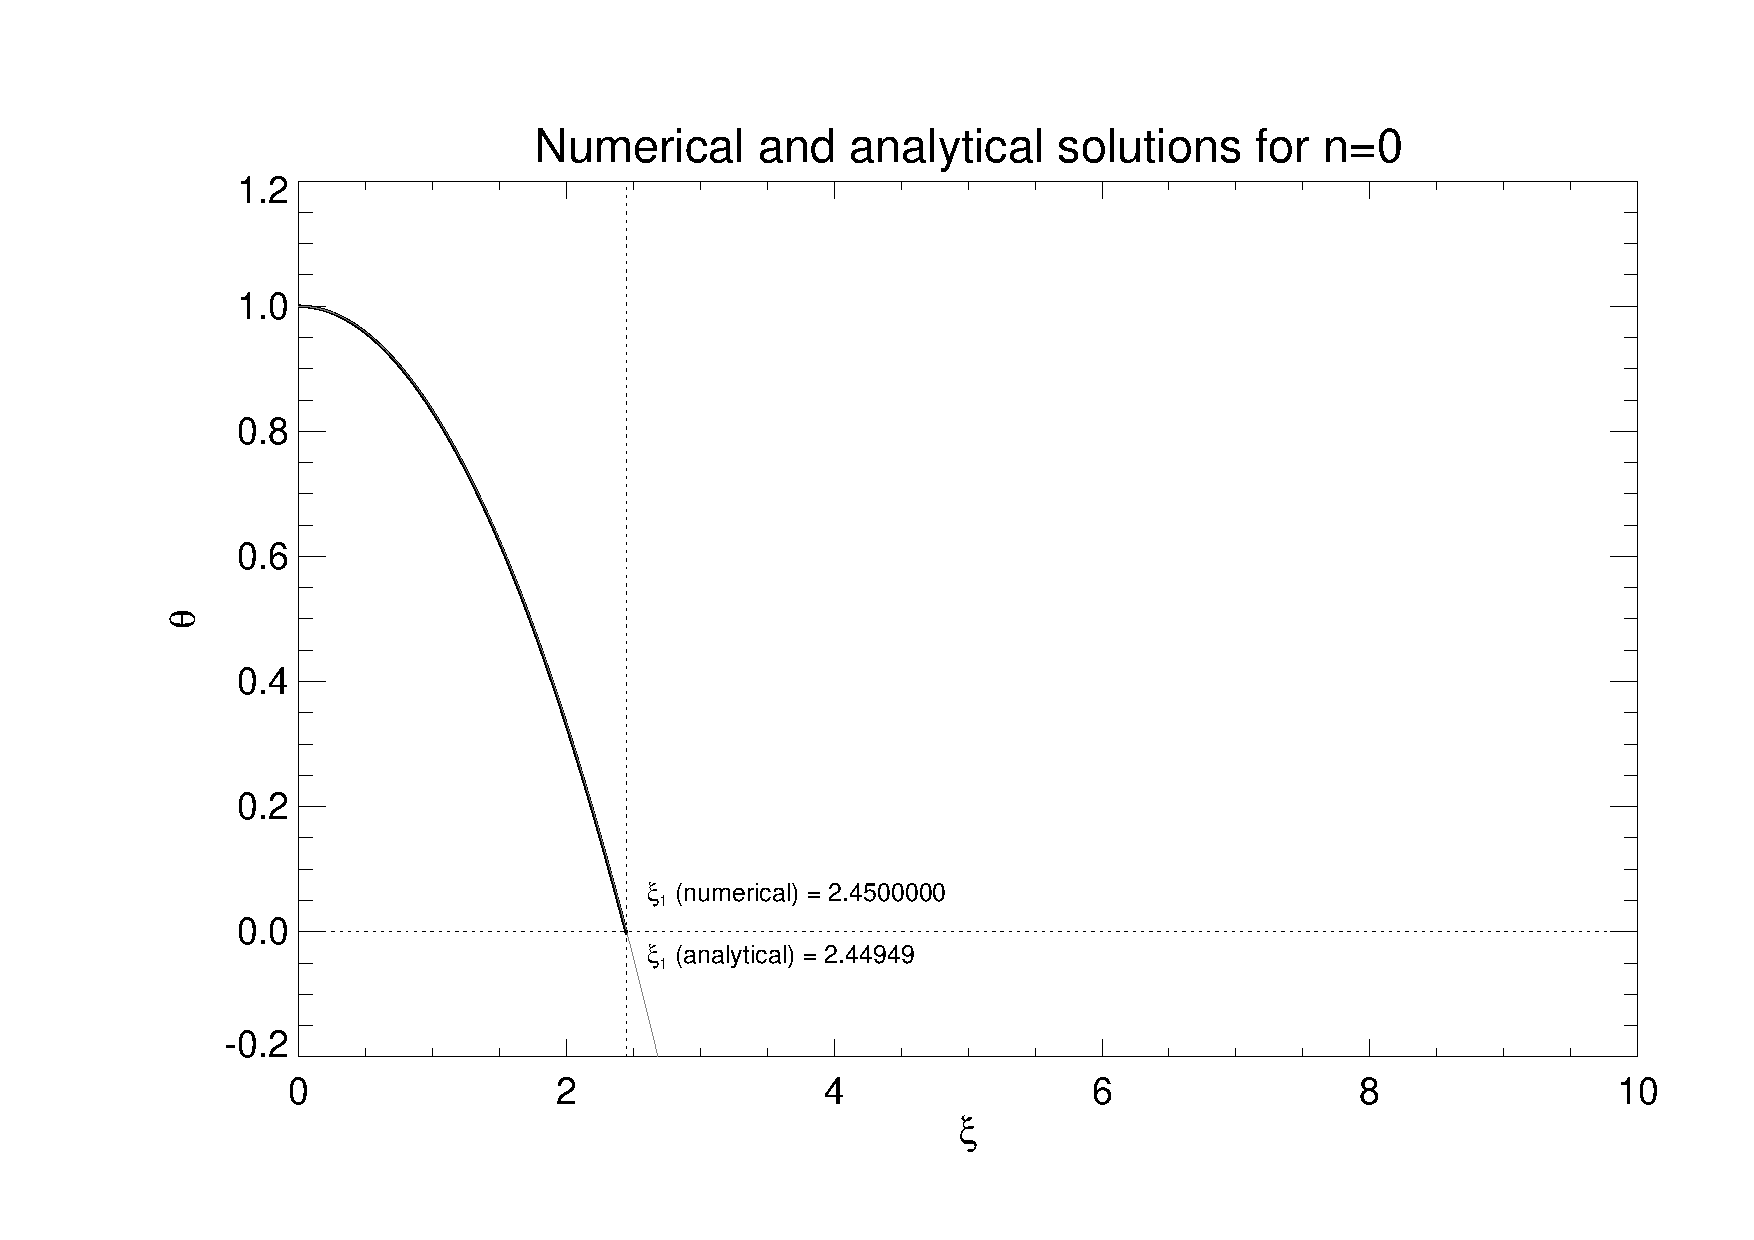
\includegraphics[scale=0.6,page=1]{stellar_part2.pdf}}

%The numerical result for $n=0$ is very close to the analytical one. %Here  $\xi_1=2.4500000$.

%\centerline{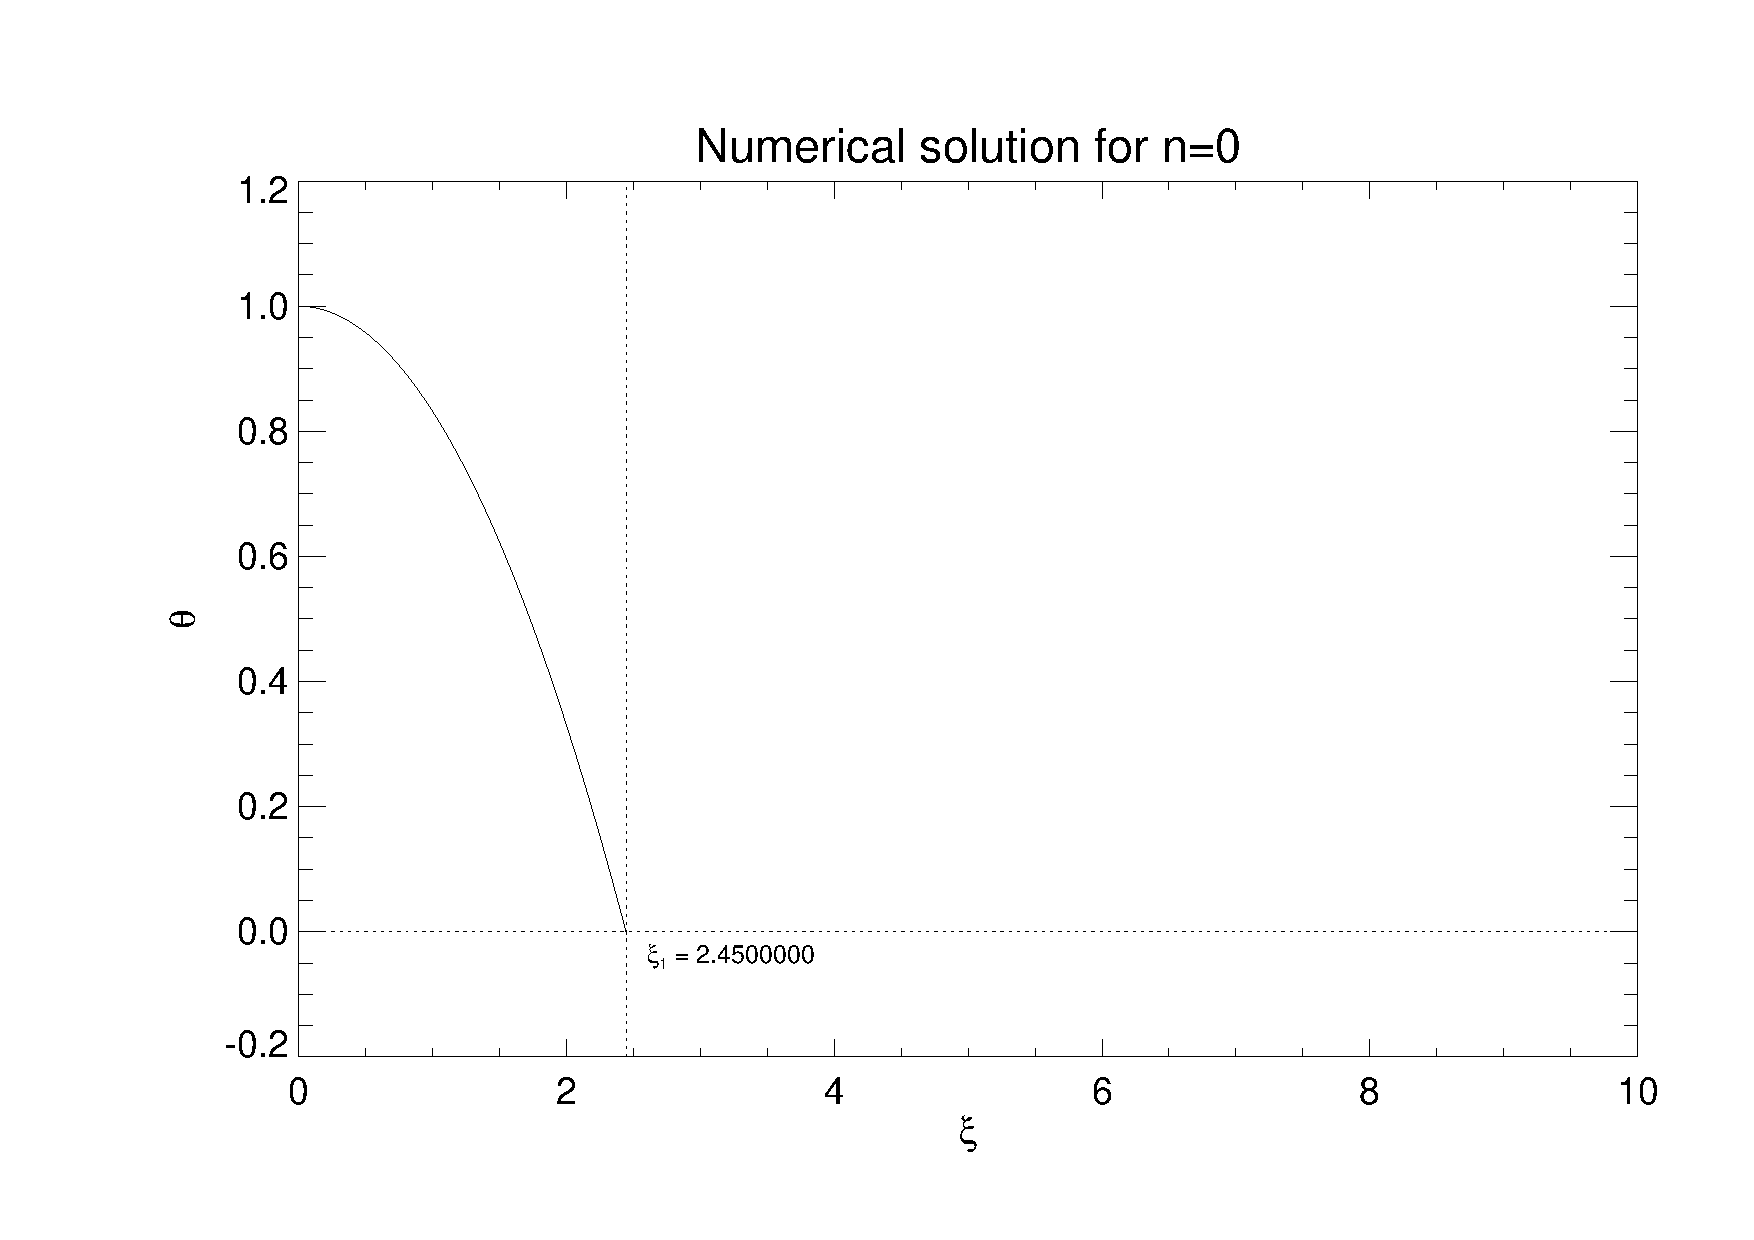
\includegraphics[scale=0.6]{stellar_part1_n0.pdf}}


%\newpage
For $n=1$ the analytical solution is
\begin{equation}
\theta(\xi)=\frac{\sin \xi}{\xi} \, .
\end{equation}

In IDL the numerical (black line) and analytical (grey line) solutions for $n=1$ look like this:

\centerline{\includegraphics[scale=0.6,page=2]{stellar_part2.pdf}}
%Now $\xi_1=\pi \approx 3.14159$ (where $\theta=0$ for the first time).

%The numerical solution is again fairly close to the analytical one:

%\centerline{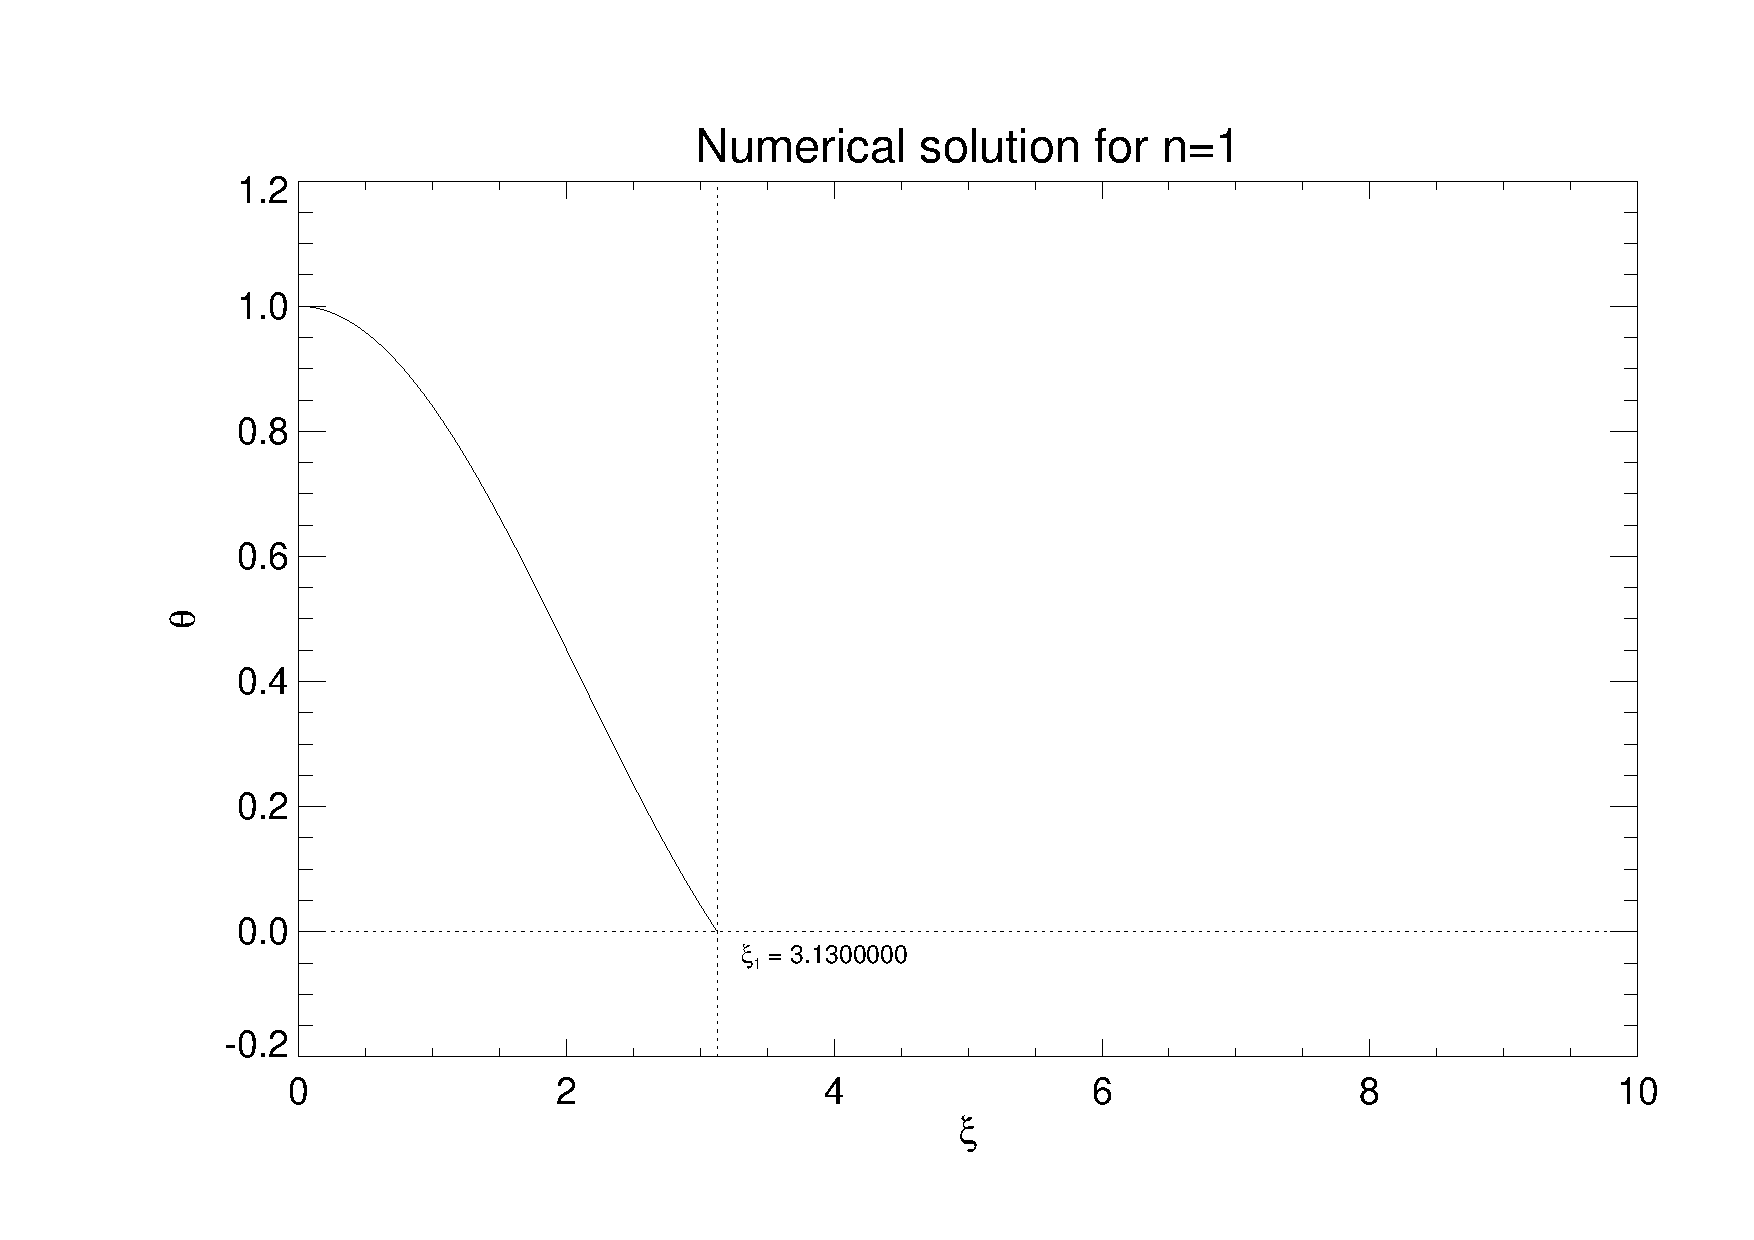
\includegraphics[scale=0.6]{stellar_part1_n1.pdf}}
%Here $\xi_1 = 3.1300000$.

\newpage
\item[\textbf{Part 3.}]

Compute $D_n$, $M_n$, $R_n$ and $B_n$ for each $n$.

\vspace{0.5cm}
\textbf{Solution}

From lecture notes we get that

\begin{equation}
R_n=\xi_1 \, ,
\end{equation}
where $\xi_1$ corresponds to the stellar radius (where $\theta = 0$).

Other constants are (again, from the lecture notes):

\begin{equation}
B_n = \frac{(3 D_n)^{\frac{3-n}{n}}}{(n+1) M_n^{\frac{n-1}{n}} R_n^{\frac{3-n}{n}}}
\end{equation}

\begin{equation}
D_n=-\left[\frac{3}{\xi_1} \left(\frac{d\theta}{d\xi}\right)_{\xi_1} \right]^{-1}
\end{equation}

\begin{equation}
M_n = -\xi_1^2 \left(\frac{d\theta}{d\xi}\right)_{\xi_1}
\end{equation}

These are solved in the program written in IDL:

\begin{scriptsize}
\begin{verbatim}
;------------------------------------------------------------------------;
; Stellar structure and evolution
; Computer assignment for advanced students
;------------------------------------------------------------------------;

;  PART III - Polytropic constants

;------------------------------------------------------------------------;
; Use the subroutine PsPlot to save results in a postscript plot 
; (written by Heikki Salo)
;------------------------------------------------------------------------;

pro PsPlot,routine,filename
	thisdir=getenv('PWD')+'/'
	psopen,/color,dir=thisdir,filename
	call_procedure,routine
	psclose		
end
;------------------------------------------------------------------------;

;------------------------------------------------------------------------;
;  MAIN PROGRAM starts here
;------------------------------------------------------------------------;
;Compute Dn, Mn, Rn and Bn for each value of n.

pro stellar_part3

;------------------------------------------------------------------------;
; Solve Lane-Emden for n=0
;------------------------------------------------------------------------;
n1=0.d0
results1=lane_emden(n1)
;Separate the results
ksi1=results1[*,0]
theta1=results1[*,1]
dtheta_dksi1=results1[*,2]

;------------------------------------------------------------------------;
; Rn (for n=0)
;------------------------------------------------------------------------;
;The program lane_emden cuts the results at theta=0, which means that
;the last term of the vector ksi is Rn

limit1=n_elements(ksi1)-1
Rn1=ksi1(limit1)
;print,theta1(limit1)
print,'Rn1(n=0)'
print,Rn1

;------------------------------------------------------------------------;
; Dn (for n=0)
;------------------------------------------------------------------------;
Dn1=-1.d0/(3.d0/Rn1*dtheta_dksi1(limit1))
print,'Dn1(n=0)'
print,Dn1

;------------------------------------------------------------------------;
; Mn (for n=0)
;------------------------------------------------------------------------;
Mn1=-Rn1^2*dtheta_dksi1(limit1)
print,'Mn1(n=0)'
print,Mn1

;------------------------------------------------------------------------;
; Bn (for n=0)
;------------------------------------------------------------------------;
;The equation would normally be:
;Bn1=(3.d0*Dn1)^((3-n1)/(3*n1))/((n1+1)*Mn^((n1-1)/n1)*Rn^((3-n1)/n1))
;n=0 is a special case, so for n->0 we define
Bn1=1.d0
print,'Bn1(n=0)'
print,Bn1

;------------------------------------------------------------------------;
; Solve Lane-Emden for n=0.5
;------------------------------------------------------------------------;
n2=0.5d0
results2=lane_emden(n2)
;Separate the results
ksi2=results2[*,0]
theta2=results2[*,1]
dtheta_dksi2=results2[*,2]

;------------------------------------------------------------------------;
; Rn (for n=0.5)
;------------------------------------------------------------------------;
limit2=n_elements(ksi2)-1
Rn2=ksi2(limit2)
print,'Rn2(n=0.5)'
print,Rn2

;------------------------------------------------------------------------;
; Dn (for n=0.5)
;------------------------------------------------------------------------;
Dn2=-1.d0/(3.d0/Rn2*dtheta_dksi2(limit2))
print,'Dn2(n=0.5)'
print,Dn2

;------------------------------------------------------------------------;
; Mn (for n=0.5)
;------------------------------------------------------------------------;
Mn2=-Rn2^2*dtheta_dksi2(limit2)
print,'Mn2(n=0.5)'
print,Mn2

;------------------------------------------------------------------------;
; Bn (for n=0.5)
;------------------------------------------------------------------------;
Bn2=(3.d0*Dn2)^((3.d0-n2)/(3.d0*n2))/((n2+1.d0)*Mn2^((n2-1.d0)/n2)*Rn2^((3.d0-n2)/n2))
print,'Bn2(n=0.5)'
print,Bn2

;------------------------------------------------------------------------;
; Solve Lane-Emden for n=1
;------------------------------------------------------------------------;
n3=1.d0
results3=lane_emden(n3)
;Separate the results
ksi3=results3[*,0]
theta3=results3[*,1]
dtheta_dksi3=results3[*,2]

;------------------------------------------------------------------------;
; Rn (for n=1)
;------------------------------------------------------------------------;
limit3=n_elements(ksi3)-1
Rn3=ksi3(limit3)
print,'Rn3(n=1)'
print,Rn3

;------------------------------------------------------------------------;
; Dn (for n=1)
;------------------------------------------------------------------------;
Dn3=-1.d0/(3.d0/Rn3*dtheta_dksi3(limit3))
print,'Dn3(n=1)'
print,Dn3

;------------------------------------------------------------------------;
; Mn (for n=1)
;------------------------------------------------------------------------;
Mn3=-Rn3^2*dtheta_dksi3(limit3)
print,'Mn3(n=1)'
print,Mn3

;------------------------------------------------------------------------;
; Bn (for n=1)
;------------------------------------------------------------------------;
Bn3=(3.d0*Dn3)^((3.d0-n3)/(3.d0*n3))/((n3+1.d0)*Mn3^((n3-1.d0)/n3)*Rn3^((3.d0-n3)/n3))
print,'Bn3(n=1)'
print,Bn3

;------------------------------------------------------------------------;
; Solve Lane-Emden for n=1.5
;------------------------------------------------------------------------;
n4=1.5d0
results4=lane_emden(n4)
;Separate the results
ksi4=results4[*,0]
theta4=results4[*,1]
dtheta_dksi4=results4[*,2]

;------------------------------------------------------------------------;
; Rn (for n=1.5)
;------------------------------------------------------------------------;
limit4=n_elements(ksi4)-1
Rn4=ksi4(limit4)
print,'Rn4(n=1.5)'
print,Rn4

;------------------------------------------------------------------------;
; Dn (for n=1.5)
;------------------------------------------------------------------------;
Dn4=-1.d0/(3.d0/Rn4*dtheta_dksi4(limit4))
print,'Dn4(n=1.5)'
print,Dn4

;------------------------------------------------------------------------;
; Mn (for n=1.5)
;------------------------------------------------------------------------;
Mn4=-Rn4^2*dtheta_dksi4(limit4)
print,'Mn4(n=1.5)'
print,Mn4

;------------------------------------------------------------------------;
; Bn (for n=1.5)
;------------------------------------------------------------------------;
Bn4=(3.d0*Dn4)^((3-n4)/(3*n4))/((n4+1.d0)*Mn4^((n4-1)/n4)*Rn4^((3.d0-n4)/n4))
print,'Bn4(n=1.5)'
print,Bn4

;------------------------------------------------------------------------;
; Solve Lane-Emden for n=2
;------------------------------------------------------------------------;
n5=2.d0
results5=lane_emden(n5)
;Separate the results
ksi5=results5[*,0]
theta5=results5[*,1]
dtheta_dksi5=results5[*,2]

;------------------------------------------------------------------------;
; Rn (for n=2)
;------------------------------------------------------------------------;
limit5=n_elements(ksi5)-1
Rn5=ksi5(limit5)
print,'Rn5(n=2)'
print,Rn5

;------------------------------------------------------------------------;
; Dn (for n=2)
;------------------------------------------------------------------------;
Dn5=-1.d0/(3.d0/Rn5*dtheta_dksi5(limit5))
print,'Dn5(n=2)'
print,Dn5

;------------------------------------------------------------------------;
; Mn (for n=2)
;------------------------------------------------------------------------;
Mn5=-Rn5^2*dtheta_dksi5(limit5)
print,'Mn5(n=2)'
print,Mn5

;------------------------------------------------------------------------;
; Bn (for n=2)
;------------------------------------------------------------------------;
Bn5=(3.d0*Dn5)^((3.d0-n5)/(3.d0*n5))/((n5+1.d0)*Mn5^((n5-1)/n5)*Rn5^((3.d0-n5)/n5))
print,'Bn5(n=2)'
print,Bn5

;------------------------------------------------------------------------;
; Solve Lane-Emden for n=2.5
;------------------------------------------------------------------------;
n6=2.5d0
results6=lane_emden(n6)
;Separate the results
ksi6=results6[*,0]
theta6=results6[*,1]
dtheta_dksi6=results6[*,2]

;------------------------------------------------------------------------;
; Rn (for n=2.5)
;------------------------------------------------------------------------;
limit6=n_elements(ksi6)-1
Rn6=ksi6(limit6)
print,'Rn6(n=2.5)'
print,Rn6

;------------------------------------------------------------------------;
; Dn (for n=2.5)
;------------------------------------------------------------------------;
Dn6=-1.d0/(3.d0/Rn6*dtheta_dksi6(limit6))
print,'Dn6(n=2.5)'
print,Dn6

;------------------------------------------------------------------------;
; Mn (for n=2.5)
;------------------------------------------------------------------------;
Mn6=-Rn6^2*dtheta_dksi6(limit6)
print,'Mn6(n=2.5)'
print,Mn6

;------------------------------------------------------------------------;
; Bn (for n=2.5)
;------------------------------------------------------------------------;
Bn6=(3.d0*Dn6)^((3.d0-n6)/(3.d0*n6))/((n6+1.d0)*Mn6^((n6-1)/n6)*Rn6^((3.d0-n6)/n6))
print,'Bn6(n=2.5)'
print,Bn6

;------------------------------------------------------------------------;
; Solve Lane-Emden for n=3
;------------------------------------------------------------------------;
n7=3.d0
results7=lane_emden(n7)
;Separate the results
ksi7=results7[*,0]
theta7=results7[*,1]
dtheta_dksi7=results7[*,2]

;------------------------------------------------------------------------;
; Rn (for n=3)
;------------------------------------------------------------------------;
limit7=n_elements(ksi7)-1
Rn7=ksi7(limit7)
print,'Rn7(n=3)'
print,Rn7

;------------------------------------------------------------------------;
; Dn (for n=3)
;------------------------------------------------------------------------;
Dn7=-1.d0/(3.d0/Rn7*dtheta_dksi7(limit7))
print,'Dn7(n=3)'
print,Dn7

;------------------------------------------------------------------------;
; Mn (for n=3)
;------------------------------------------------------------------------;
Mn7=-Rn7^2*dtheta_dksi7(limit7)
print,'Mn7(n=3)'
print,Mn7

;------------------------------------------------------------------------;
; Bn (for n=3)
;------------------------------------------------------------------------;
Bn7=(3.d0*Dn7)^((3.d0-n7)/(3.d0*n7))/((n7+1.d0)*Mn7^((n7-1)/n7)*Rn7^((3.d0-n7)/n7))
print,'Bn7(n=3)'
print,Bn7

;------------------------------------------------------------------------;
; Solve Lane-Emden for n=3.5
;------------------------------------------------------------------------;
n8=3.5d0
results8=lane_emden(n8)
;Separate the results
ksi8=results8[*,0]
theta8=results8[*,1]
dtheta_dksi8=results8[*,2]

;------------------------------------------------------------------------;
; Rn (for n=3.5)
;------------------------------------------------------------------------;
limit8=n_elements(ksi8)-1
Rn8=ksi8(limit8)
print,'Rn8(n=3.5)'
print,Rn8

;------------------------------------------------------------------------;
; Dn (for n=3.5)
;------------------------------------------------------------------------;
Dn8=-1.d0/(3.d0/Rn8*dtheta_dksi8(limit8))
print,'Dn8(n=3.5)'
print,Dn8

;------------------------------------------------------------------------;
; Mn (for n=3.5)
;------------------------------------------------------------------------;
Mn8=-Rn8^2*dtheta_dksi8(limit8)
print,'Mn8(n=3.5)'
print,Mn8

;------------------------------------------------------------------------;
; Bn (for n=3.5)
;------------------------------------------------------------------------;
Bn8=(3.d0*Dn8)^((3.d0-n8)/(3.d0*n8))/((n8+1.d0)*Mn8^((n8-1)/n8)*Rn8^((3.d0-n8)/n8))
print,'Bn8(n=3.5)'
print,Bn8

;------------------------------------------------------------------------;
; Solve Lane-Emden for n=4
;------------------------------------------------------------------------;
n9=4.d0
results9=lane_emden(n9)
;Separate the results
ksi9=results9[*,0]
theta9=results9[*,1]
dtheta_dksi9=results9[*,2]

;------------------------------------------------------------------------;
; Rn (for n=4)
;------------------------------------------------------------------------;
limit9=n_elements(ksi9)-1
Rn9=ksi9(limit9)
print,'Rn9(n=4)'
print,Rn9

;------------------------------------------------------------------------;
; Dn (for n=4)
;------------------------------------------------------------------------;
Dn9=-1.d0/(3.d0/Rn9*dtheta_dksi9(limit9))
print,'Dn9(n=4)'
print,Dn9

;------------------------------------------------------------------------;
; Mn (for n=4)
;------------------------------------------------------------------------;
Mn9=-Rn9^2*dtheta_dksi9(limit9)
print,'Mn9(n=4)'
print,Mn9

;------------------------------------------------------------------------;
; Bn (for n=4)
;------------------------------------------------------------------------;
Bn9=(3.d0*Dn9)^((3.d0-n9)/(3.d0*n9))/((n9+1.d0)*Mn9^((n9-1)/n9)*Rn9^((3.d0-n9)/n9))
print,'Bn9(n=4)'
print,Bn9

;------------------------------------------------------------------------;
; Solve Lane-Emden for n=4.5
;------------------------------------------------------------------------;
n10=4.5d0
results10=lane_emden(n10)
;Separate the results
ksi10=results10[*,0]
theta10=results10[*,1]
dtheta_dksi10=results10[*,2]

;------------------------------------------------------------------------;
; Rn (for n=4.5)
;------------------------------------------------------------------------;
limit10=n_elements(ksi10)-1
Rn10=ksi10(limit10)
print,'Rn10(n=4.5)'
print,Rn10

;------------------------------------------------------------------------;
; Dn (for n=4.5)
;------------------------------------------------------------------------;
Dn10=-1.d0/(3.d0/Rn10*dtheta_dksi10(limit10))
print,'Dn10(n=4.5)'
print,Dn10

;------------------------------------------------------------------------;
; Mn (for n=4.5)
;------------------------------------------------------------------------;
Mn10=-Rn10^2*dtheta_dksi10(limit10)
print,'Mn10(n=4.5)'
print,Mn10

;------------------------------------------------------------------------;
; Bn (for n=4.5)
;------------------------------------------------------------------------;
Bn10=(3.d0*Dn10)^((3.d0-n10)/(3.d0*n10))/((n10+1.d0)*Mn10^((n10-1)/n10)*Rn10^((3.d0-n10)/n10))
print,'Bn10(n=4.5)'
print,Bn10

;------------------------------------------------------------------------;
; Solve Lane-Emden for n=5
;------------------------------------------------------------------------;
n11=5.d0
results11=lane_emden(n11)
;Separate the results
ksi11=results11[*,0]
theta11=results11[*,1]
dtheta_dksi11=results11[*,2]

;------------------------------------------------------------------------;
; Rn (for n=5)
;------------------------------------------------------------------------;
limit11=n_elements(ksi11)-1
Rn11=ksi11(limit11)
print,'Rn11(n=5)'
print,Rn11

;------------------------------------------------------------------------;
; Dn (for n=5)
;------------------------------------------------------------------------;
Dn11=-1.d0/(3.d0/Rn11*dtheta_dksi11(limit11))
print,'Dn11(n=5)'
print,Dn11

;------------------------------------------------------------------------;
; Mn (for n=5)
;------------------------------------------------------------------------;
Mn11=-Rn11^2*dtheta_dksi11(limit11)
print,'Mn11(n=5)'
print,Mn11

;------------------------------------------------------------------------;
; Bn (for n=5)
;------------------------------------------------------------------------;
Bn11=(3.d0*Dn11)^((3.d0-n11)/(3.d0*n11))/((n11+1.d0)*Mn11^((n11-1)/n11)*Rn11^((3.d0-n11)/n11))
print,'Bn11(n=5)'
print,Bn11

end

;--------------------------------------------------------------------;
; Save the results to a PostScript file using PsPlot
;--------------------------------------------------------------------;

pro plot_everything
PsPlot, 'stellar_part3', 'stellar_part3.ps'
end
\end{verbatim}
\end{scriptsize}

\newpage
\vspace{0.5cm}
\textbf{Results}

Table of the final results:

\vspace{0.5cm}
\begin{tabular}{|l|c|c|c|c|}
\hline
$n$ & $D_n$ & $M_n$ & $R_n$ & $B_n$ \\
\hline
$0.0$ & $0.99959184$ & $4.8980408$ & $2.4490000$ & $1.0000000$ \\
%\hline
$0.5$ & $1.8338162$ & $3.7885081$ & $2.7520000$ & $0.27432365$ \\
%\hline
$1.0$ & $3.2890093$ & $3.1406349$ & $3.1410000$ & $0.23314443$ \\
%\hline
$1.5$ & $5.9851064$ & $2.7126838$ & $3.6520000$ & $0.20564929$ \\
%\hline
$2.0$ & $11.395406$ & $2.4094405$ & $4.3510000$ & $0.18546755$ \\
%\hline
$2.5$ & $23.395297$ & $2.1854552$ & $5.3530000$ & $0.16965657$ \\
%\hline
$3.0$ & $54.164361$ & $2.0164105$ & $6.8940000$ & $0.15663448$ \\
%\hline
$3.5$ & $152.94777$ & $1.8886915$ & $9.5340000$ & $0.14543875$ \\
%\hline
$4.0$ & $623.61190$ & $1.7953612$ & $14.976000$ & $0.13539276$ \\
%\hline
$4.5$ & $6230.1945$ & $1.7359810$ & $31.895000$ & $0.12587534$ \\
%\hline
$5.0$ & ? & ? & ? & ? \\
\hline
\end{tabular}

\vspace{0.5cm}
Solving the polytropic constants for all the other polytropes except $n=5$ was rather straightforward, but in the $n=5$ case the results didn't make any sense.

If we solve the Lane-Emden equation separately for $n=5$ between $0 \leq \xi \leq 300$ and plot the results, we see that $\theta = 0$ is never reached (increasing $\xi$ doesn't seem to help, the $\theta = 0$ limit is never crossed). This must mean that $R_n \to \infty$ when $\theta \to 0$.

%\vspace{0.5cm}
\centerline{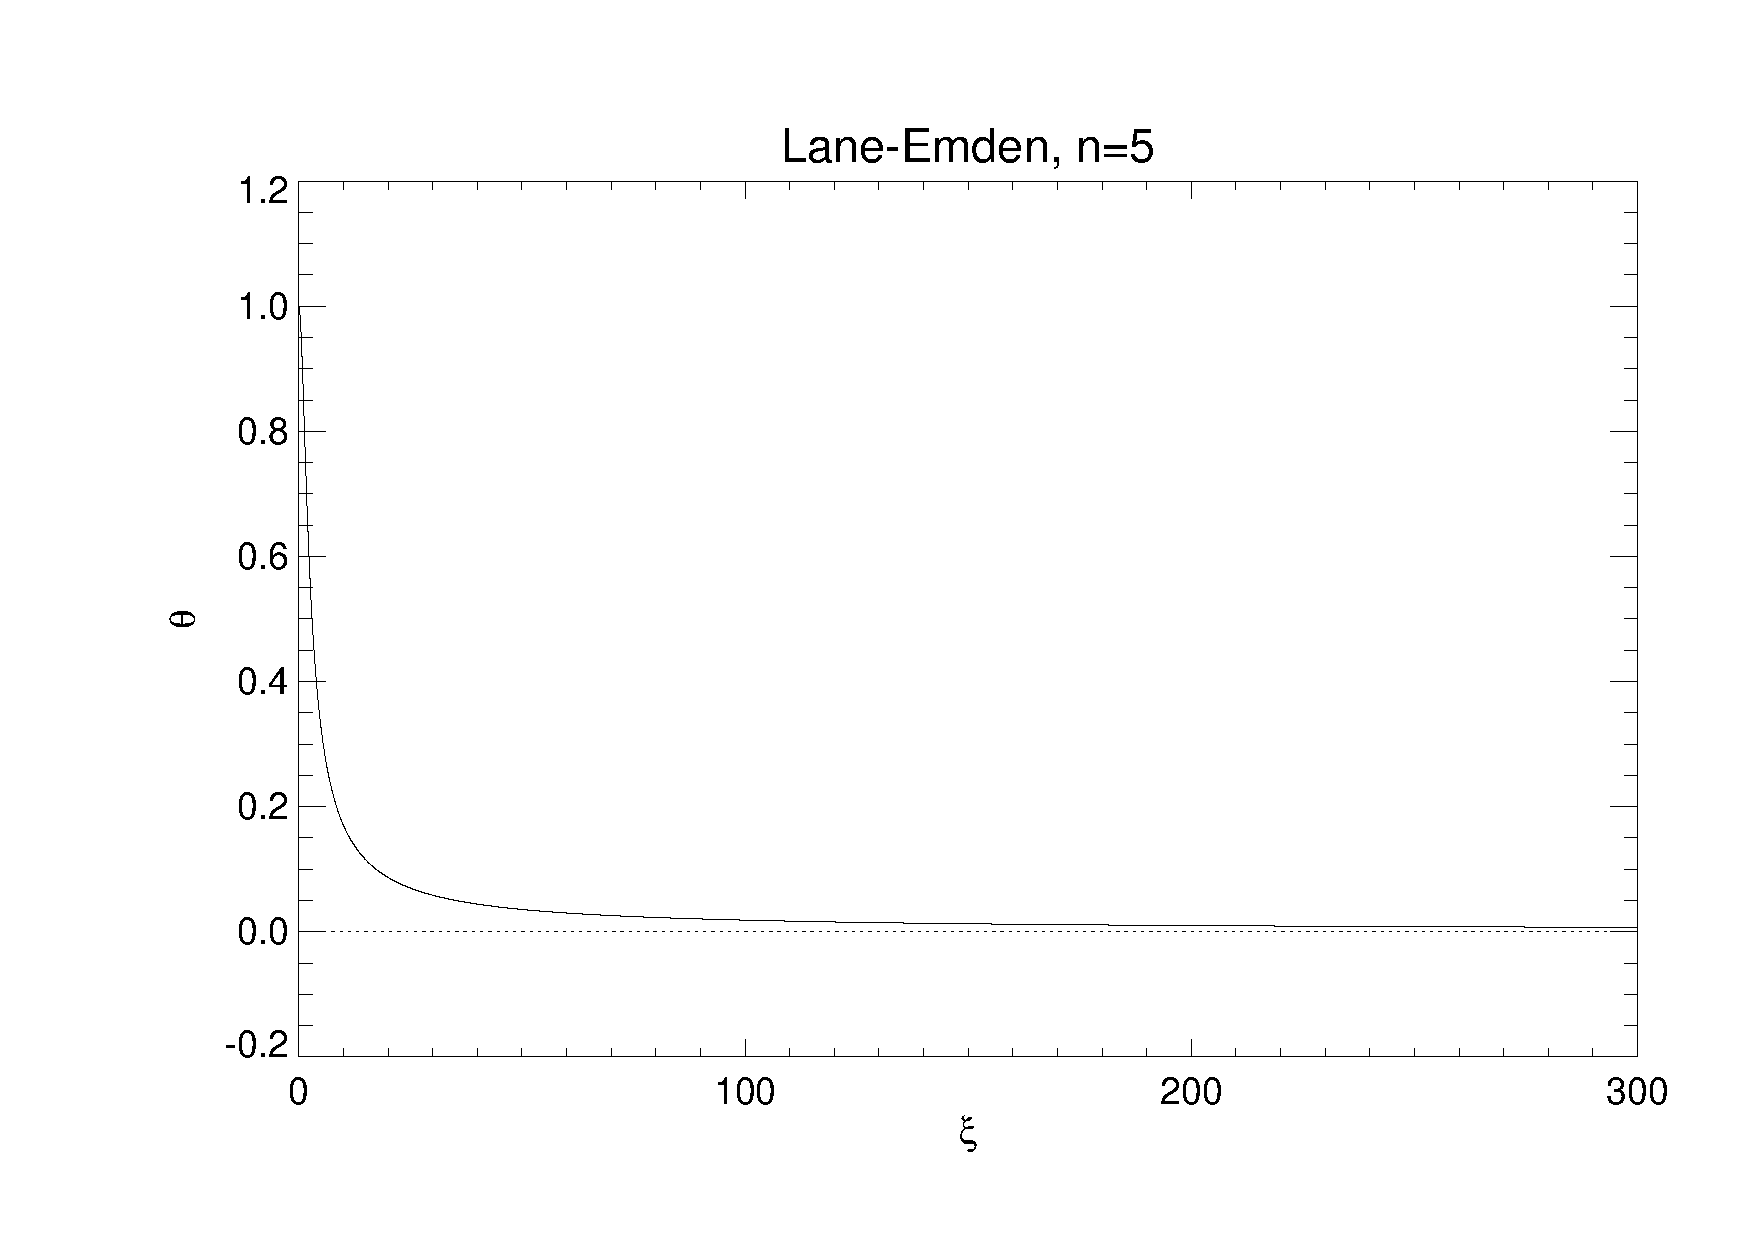
\includegraphics[scale=0.6]{stellar_poly5.pdf}}
\vspace*{0.5cm}

The analytical solution for $n=5$

\begin{equation}
\theta(\xi) = (1+ \frac{ \xi^2}{3})^{-\frac{1}{2}} 
\end{equation}
yields similar results

\centerline{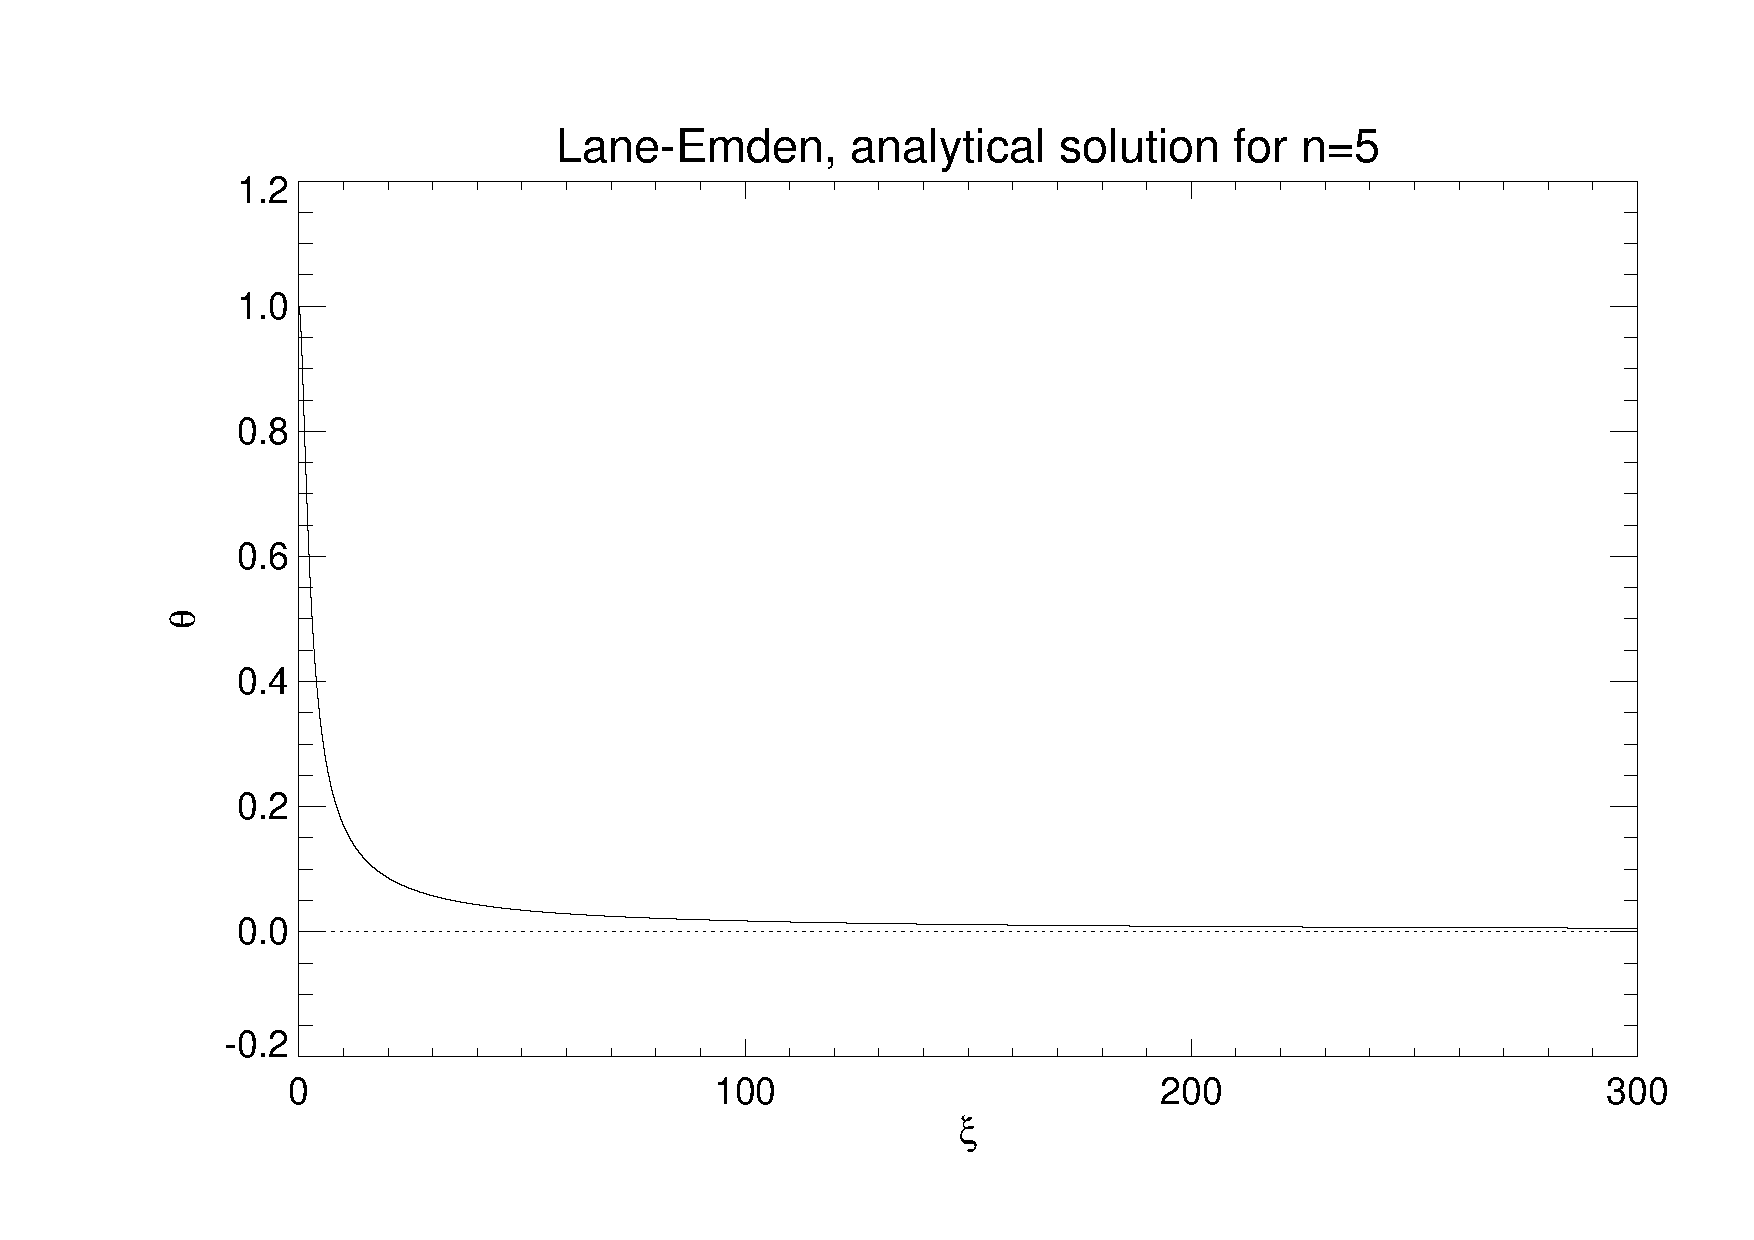
\includegraphics[scale=0.6]{analytical5.pdf}}

\newpage

\textbf{The failed iteration for $\mathbf{n \to 5}$}

%Here are the futile efforts for solving the polytropic constants for n=5 so far:

%\begin{scriptsize}
%\begin{verbatim}
%Here was the program code, check part IIIc
%\end{verbatim}
%\end{scriptsize}

This method didn't succeed, but I'll document the efforts anyway for the purpose of maybe gaining some sympathy points.

I thought I could solve $R_n$ for different values of $n=4.9$, $n=4.99$, $n=4.999$ and so on with a handy iteration loop (as long as $n<5$, $R_n$ should be a finite number), and then use the results for solving the other constants. I would then see what values the polytropic constants are approaching as $R_n \to \infty $. However, this method would require that I would be able to increase the integration range ridiculously high. 

Only the $n=4.9$ graph reached $\theta=0$ before $\xi=300$, none of the following ones did. The magical $\xi=300$ limit is a result of trial and error. If I increased the number of points in the $\theta(\xi)$ -vector to over 30000, the computer freezed while trying to solve the Lane-Emden equation. Increasing the range of $\xi$ could only be achieved by increasing the step size, but that led me nowhere, as the accuracy dropped wildly.
%I have no idea how else can I solve the constants numerically. Unless I understood everything wrong and this part was supposed to be solved analytically. But that I cannot do, because I am an idiot with no math skills.

I have concluded that my efforts were pointless and stupid, as I could just have set $n=5$ and $R_n$ as incredibly large.

\vspace{0.5cm}
\textbf{Solution: The program in IDL}

\begin{scriptsize}
\begin{verbatim}
;------------------------------------------------------------------------;
; Stellar structure and evolution
; Computer assignment for advanced students
;------------------------------------------------------------------------;
; Solving the polytropic constants for n=5

pro constants_n5

n=5

;------------------------------------------------------------------------;
;  Rn
;------------------------------------------------------------------------;
;Instead of solving the Rn from Lane-Emden equation like in the
;previous versions, just set Rn to be ridiculously large

;Rn=10.d0^38
Rn=10.d0^99

;------------------------------------------------------------------------;
; (dtheta/dksi)_ksi1
;------------------------------------------------------------------------;
;The derivative of the analytical solution (at ksi=Rn) is:

dtheta_dksi=-0.5d0*(1.d0+Rn^2/3.d0)^(-1.5d0)*2.d0/3*Rn

;------------------------------------------------------------------------;
; Dn
;------------------------------------------------------------------------;
Dn=-1.d0/(3.d0/Rn*dtheta_dksi)
print,'Dn'
print,Dn

print,'Compare with: infinity'

;------------------------------------------------------------------------;
; Mn
;------------------------------------------------------------------------;
Mn=-Rn^2*dtheta_dksi
print,'Mn'
print,Mn

print,'Compare with:'
print,sqrt(3.d0)

;------------------------------------------------------------------------;
; Bn
;------------------------------------------------------------------------;
Bn=(3.d0*Dn)^((3.d0-n)/(3.d0*n))/((n+1.d0)*Mn^((n-1.d0)/n)*Rn^((3.d0-n)/n))
print,'Bn'
print,Bn

print,'Compare with:'
print,(3.d0^(1.d0/3)*6.d0)^(-1.d0)

end
\end{verbatim}
\end{scriptsize}

\vspace{0.5cm}
\textbf{Final results for n=5}

Using the analytical solution, and setting $R_n$ as very large (and checking if the values change when $R_n$ increases), I got the following results:

$$D_n=1.9245009 \cdot 10^{296}$$
This value increased every time I increased $R_n$, so it is safe to assume that $D_n \to \infty$.

$$M_n=1.7320508$$
I compared this with Mikko's analytical solution $M_n=\sqrt{3}$ and it was the same result.

$$B_n=0.11556021$$
Mikko got the result $M_n=(3^{\frac{1}{3}} \cdot 6)^{-1}$ which is the same thing, although mathematically more beautiful.



%\newpage
%\vspace{0.5cm}
%\textbf{Results}

Updated table of the final results:

\vspace{0.5cm}
\begin{tabular}{|l|c|c|c|c|}
\hline
$n$ & $D_n$ & $M_n$ & $R_n$ & $B_n$ \\
\hline
$0.0$ & $0.99959184$ & $4.8980408$ & $2.4490000$ & $1.0000000$ \\
%\hline
$0.5$ & $1.8338162$ & $3.7885081$ & $2.7520000$ & $0.27432365$ \\
%\hline
$1.0$ & $3.2890093$ & $3.1406349$ & $3.1410000$ & $0.23314443$ \\
%\hline
$1.5$ & $5.9851064$ & $2.7126838$ & $3.6520000$ & $0.20564929$ \\
%\hline
$2.0$ & $11.395406$ & $2.4094405$ & $4.3510000$ & $0.18546755$ \\
%\hline
$2.5$ & $23.395297$ & $2.1854552$ & $5.3530000$ & $0.16965657$ \\
%\hline
$3.0$ & $54.164361$ & $2.0164105$ & $6.8940000$ & $0.15663448$ \\
%\hline
$3.5$ & $152.94777$ & $1.8886915$ & $9.5340000$ & $0.14543875$ \\
%\hline
$4.0$ & $623.61190$ & $1.7953612$ & $14.976000$ & $0.13539276$ \\
%\hline
$4.5$ & $6230.1945$ & $1.7359810$ & $31.895000$ & $0.12587534$ \\
%\hline
$5.0$ & $1.9245009 \cdot 10^{296}$ ($\infty$) & $M_n=1.7320508$ & $\infty$ & $0.11556021$ \\
\hline
\end{tabular}

\newpage
\item[\textbf{Part 4}] A sophisticated solar model can be found at 
\begin{verbatim}
http://www.sns.ias.edu/~jnb/SNdata/Export/BS2005/bs05_agsop.dat 
(Bachall et al.2005).
\end{verbatim}

Compare the profiles $\log\rho$, $M/M_{\odot}$, $\log P$ and $\log T$ as a function of $R/R_{\odot}$ of this complicated model with those of an $n=3$ polytrope considering that the composition of the Sun is uniform with $\mu = 0.61$.

\vspace{0.5cm}
\textbf{Results}

%Based on the given data file, the profiles of the complicated solar model look like

IDL plots of the profiles for $n=3$ polytrope (gray line) and the solar model (black line):

\centerline{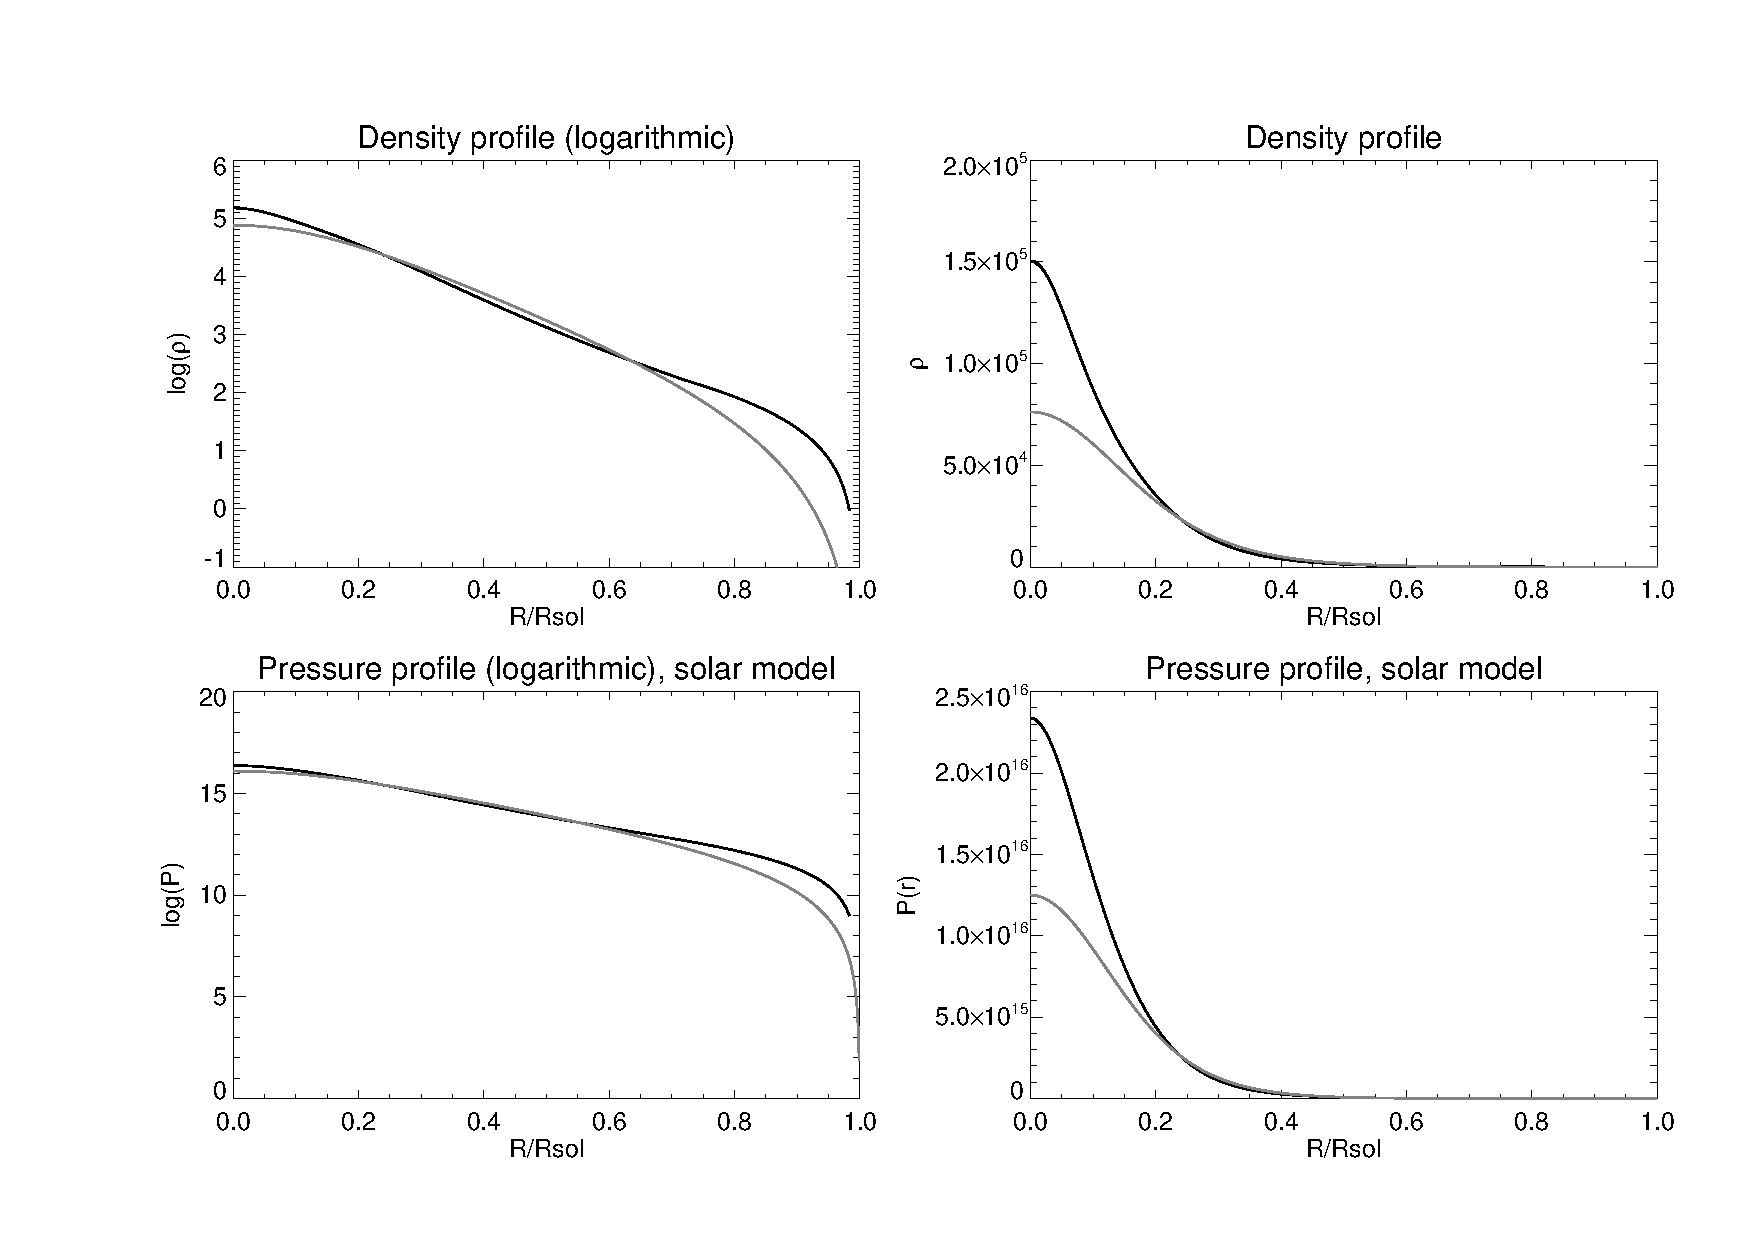
\includegraphics[scale=0.6,page=1]{compare2.pdf}}

\centerline{\includegraphics[scale=0.6,page=2]{compare2.pdf}}

%\vspace{0.5cm}
%\textbf{n=3 polytrope}

%Based on the solved Lane-Emden equation, the corresponding profiles for the n=3 polytrope are

%\centerline{\includegraphics[scale=0.6,page=2]{compare.pdf}}

%\centerline{\includegraphics[scale=0.6,page=3]{compare.pdf}}

%The density profiles are otherwise similar, except that in the polytropic model the density approaches zero at the surface. The sophisticated model is cut short just before the surface.

%The profiles of mass, pressure and temperature are also quite closely the same, except that the central pressure that I calculated is smaller than in the solar model.

\textbf{Central pressure, temperature and density for the models}

From the lecture notes I found that the pressure at the center of a polytropic star is

\begin{equation}
P_c=(4\pi)^{1/3} B_n G M^{2/3} \rho_c^{4/3} \, ,
\end{equation}

and I got $P_c=1.2503143 \cdot 10^{16}$ Pa as a result. In the solar model the pressure was $P_c=2.33800 \cdot 10^{16}$ Pa at the point closest to $R=0$ in the data file.

The central density is
\begin{equation}
\rho_c=D_n \frac{M_{\odot}}{\frac{4\pi}{3}R_{\odot}^3} \, ,
\end{equation}
%rho_c=Dn*Msol/Vsol

which was $\rho_c=76277.871 \text{kg}/\text{m}^3$ according to my model. In the solar model the central density was $\rho_c=150500.00\text{kg}/\text{m}^3$.

Finally, the central temperature is
\begin{equation}
T_c=\frac{\mu P_c}{\textit{R}\rho_c}
\end{equation}

which was $T_c=1.2122072\cdot10^7$K according to my model, and $T_c=1.54800\cdot10^7$K according to the solar model.

%\vspace{1cm}
\newpage
\textbf{IDL code for comparing the profiles}

\begin{scriptsize}
\begin{verbatim}
;------------------------------------------------------------------------;
; Stellar structure and evolution
; Computer assignment for advanced students
;------------------------------------------------------------------------;
; Final part - compare to a more realistic solar model
;------------------------------------------------------------------------;
; Use the subroutine PsPlot to save results in a postscript plot 
; (written by Heikki Salo)
;------------------------------------------------------------------------;
pro PsPlot,routine,filename
	thisdir=getenv('PWD')+'/'
	psopen,/color,dir=thisdir,filename
	call_procedure,routine
	psclose		
end
;------------------------------------------------------------------------;

;------------------------------------------------------------------------;
; MAIN PROGRAM starts here
;------------------------------------------------------------------------;
pro compare

;------------------------------------------------------------------------;
; Read data from bs05_agsop.dat -file
; 12 columns, 1284 rows
;------------------------------------------------------------------------;

;create empty array
data=fltarr(12,1284)
;open the data file
openr,lun,'bs05_agsop.dat',/get_lun
;read data
readf,lun,data
;close the file
close,/all
;check the data array
help,data
;print,data

;Separate the columns that are needed

mass=reform(data(0,*))
;help,mass
;print,mass

radius=reform(data(1,*))
;help,radius
;print,radius


temperature=alog10(reform(data(2,*)))
;help,temperature
;print,temperature
;Central temperature:
temperature_c=data(2,0)
print,'Central temperature (K)'
print,temperature_c

;Central density:
density_c=data(3,0)*1000.d0
print,'Central density (kg/m^3)'
print,density_c
;Density:
density=reform(data(3,*))*1000.d0
density_log=alog10(density)
;help,density
;print,density

pressure=reform(data(4,*))*0.1d0
pressure_log=alog10(pressure)
;Central pressure
pressure_c=data(4,0)*0.1d0
print,'Central pressure (Pa)'
print,pressure_c
;help,pressure
;print,pressure

;------------------------------------------------------------------------;
; Solar model:
; log(rho) as a function of R/Rsol
;------------------------------------------------------------------------;
;!p.multi=[0,2,2]
;nwin
;plot,radius,density_log,xtitle='R/Rsol',ytitle='log(!9r!X!N)',title='Density 
profile (logarithmic), solar model';,yrange=[-10,0]

;Non-logarithmic density
;nwin
;plot,radius,density,xtitle='R/Rsol',ytitle='!9r!X!N(r)',title='Density 
profile, solar model';,yrange=[-10,0]

;------------------------------------------------------------------------;
; Solar model:
; log(P) as a function of R/Rsol
;------------------------------------------------------------------------;
;nwin
;plot,radius,pressure_log,xtitle='R/Rsol',ytitle='log(P)',title='Pressure 
profile (logarithmic), solar model'

;Non-logarithmic pressure
;nwin
;plot,radius,pressure,xtitle='R/Rsol',ytitle='P(r)',title='Pressure profile, 
solar model'

;------------------------------------------------------------------------;
; Solar model:
; M/Msol as a function of R/Rsol
;------------------------------------------------------------------------;
;nwin
;plot,radius,mass,xtitle='R/Rsol',ytitle='M/Msol',title='Mass profile, solar 
model'

;------------------------------------------------------------------------;
; Solar model:
; log(T) as a function of R/Rsol
;------------------------------------------------------------------------;
;nwin
;plot,radius,temperature,xtitle='R/Rsol',ytitle='log(T)',title='Temperature 
profile (logarithmic), solar model'

;------------------------------------------------------------------------;
; Profiles for n=3 polytrope
;------------------------------------------------------------------------;

; Solve the Lane-Emden equation for n=3
n=3.d0
results=lane_emden(n)
ksi=results[*,0]
theta=results[*,1]
dtheta_dksi=results[*,2]

; Solve Rn
Rn=ksi(n_elements(ksi)-1)
print,'Rn'
print,Rn

; Solve Mn
Mn=-Rn^2*dtheta_dksi(n_elements(ksi)-1)
print,'Mn'
print,Mn

; Solve Dn
Dn=-(3.d0/Rn*dtheta_dksi(n_elements(ksi)-1))^(-1.d0)
print,'Dn'
print,Dn

; Solve Bn
Bn=(3.d0*Dn)^((3.d0-n)/(3*n))/((n+1.d0)*Mn^((n-1.d0)/n)*Rn^((3.d0-n)/n))
print,'Bn'
print,Bn

;-----------------------------------------------------------------------;
; n=3: Density profile
;-----------------------------------------------------------------------;
; Transform theta(ksi) -> rho(r/R)
; r/R = ksi/Rn and rho/rho_c = theta^n

; Solar mass (in kg)
Msol=1.9891d0*10.d0^30.d0
; Solar radius (in m)
Rsol=6.955d0*10.d0^8
; Solar volume (in m^3)
Vsol=4.d0/3*!dpi*Rsol^3
; Central density
rho_c=Dn*Msol/Vsol
print,'Central density from n3 (kg/m^3)'
print,rho_c

; Relative radius r/R
radius_n3=ksi/Rn

; Density rho
densityn3=theta^n*rho_c
; log(rho)
density_n3=alog10(densityn3)

; Plot (r,rho)
;nwin
;plot,radius_n3,density_n3,title='Density profile (logarithmic), n=3 polytrope',
xtitle='r/Rsol',ytitle='log(!9r!X!N)';,yrange=[-10,0]

;----------------------------------------------------------------------;
; ABSOLUTE density rho (kg/m^3)
;----------------------------------------------------------------------;
;Absolute density = (rho/rho_c)*rho_c
rho=densityn3;*rho_c

;Plot rho and compare with lecture notes
;nwin
;plot,radius_n3,densityn3,title='Density profile, n=3 polytrope',
xtitle='r/Rsol',ytitle='!9r!X(r)!N'

;-----------------------------------------------------------------------;
; ABSOLUTE radius (m)
;-----------------------------------------------------------------------;
Rabs=radius_n3*Rsol

;-----------------------------------------------------------------------;
; n=3: Mass profile
;-----------------------------------------------------------------------;

;Integrate from density profile
;dM=rho(r)*4*pi*r^2*dr

mass_n3=radius_n3*0.d0
i=1
while i lt n_elements(radius_n3) do begin
  dr=Rabs[i]-Rabs[i-1]
  mass_n3[i]=mass_n3(i-1)+rho[i]*4.d0*!dpi*Rabs[i]^2*dr
  i=i+1
endwhile

; Scale the mass to M/Msol
massn3=mass_n3/max(mass_n3)

;print,mass_n3
;Plot this after the pressure profiles
;plot,radius_n3,massn3,title='Mass profile, n=3 polytrope',xtitle='r/Rsol',ytitle='M/Msol'

;-----------------------------------------------------------------------;
; n=3: Pressure profile
;-----------------------------------------------------------------------;
;Gravitational constant (m^3/(kg*s^2))
G=6.67408d0*10^(-11.d0)

;Central pressure
press_c=(4.d0*!dpi)^(1.d0/3)*Bn*G*Msol^(2.d0/3)*rho_c^(4.d0/3)
print,'Central pressure (Pa)'
print,press_c

;-----------------------------------------------------------------------;
; Solve the pressure profile from polytropic eq. of state  P=K*rho^gamma, 
; where gamma=1+1/n is the adiabatic index
;-----------------------------------------------------------------------;

;Adiabatic index
gamma=1.d0+1.d0/n

;Constant K
K=(4.d0*!dpi*G/(n+1.d0)^n*(G*Msol/Mn)^(n-1.d0)*(Rsol/Rn)^(3.d0-n))^(1.d0/n)

;Polytropic eq. of state
press_n3=K*rho^gamma

;log(P)
pressn3=alog10(press_n3)

;nwin
;plot,radius_n3,pressn3,title='Pressure profile (logarithmic), n=3 polytrope',xtitle='r/Rsol',ytitle='log(P)'

;nwin
;plot,radius_n3,press_n3,title='Pressure profile, n=3 polytrope',xtitle='r/Rsol',ytitle='P(r)'

;Plot the mass profile now
;nwin
;plot,radius_n3,massn3,title='Mass profile, n=3 polytrope',xtitle='r/Rsol',ytitle='M/Msol'

;-----------------------------------------------------------------------;
; n=3: Temperature profile
;-----------------------------------------------------------------------;
;Assume that the gas in Sun is non-degenerate -> ideal gas
;P=RR/mu*rho*T -> T=P*mu/(RR*rho)

;Specific ideal gas constant RR (J/(mol*K))
;RR=kB/mH (from the lectures)
RR=1.3806488*10^(-23.d0)/(1.008d0*1.660539*10.d0^(-27.d0))
print,'RR'
print,RR

;Ratio of ions and electrons
mu=0.61d0

;Temperature
temp_n3=press_n3*mu/(RR*rho)

;log(T)
tempn3=alog10(temp_n3)

;plot,radius_n3,tempn3,title='Temperature profile (logarithmic), n=3
;polytrope',xtitle='r/Rsol',ytitle='log(T)'

;Central temperature Tc
mu=0.61d0
Tc_n3=mu*press_c/(RR*rho_c)
print,'Central temperature from n3'
print,Tc_n3

;------------------------------------------------------------------------;
; COMBINED FINAL PLOTS
;------------------------------------------------------------------------;

;------------------------------------------------------------------------;
; log(rho) as a function of R/Rsol
;------------------------------------------------------------------------;
!p.multi=[0,2,2]
nwin
plot,radius,density_log,xtitle='R/Rsol',ytitle='log(!9r!X!N)',title='Density 
profile (logarithmic)',thick=3;,yrange=[-10,20]
oplot,radius_n3,density_n3,col=130,thick=3

nwin
plot,radius,density,xtitle='R/Rsol',ytitle='!9r!X!N',title='Density profile',
thick=3;,yrange=[-10,20]
oplot,radius_n3,densityn3,col=130,thick=3

;------------------------------------------------------------------------;
; log(P) as a function of R/Rsol
;------------------------------------------------------------------------;
nwin
plot,radius,pressure_log,xtitle='R/Rsol',ytitle='log(P)',title='Pressure profile 
(logarithmic), solar model',thick=3;,yrange=[0,30]
oplot,radius_n3,pressn3,col=130,thick=3

;Non-logarithmic pressure
nwin
plot,radius,pressure,xtitle='R/Rsol',ytitle='P(r)',title='Pressure profile, 
solar model',thick=3;,yrange=[0,2*10^19]
oplot,radius_n3,press_n3,col=130,thick=3

;------------------------------------------------------------------------;
; M/Msol as a function of R/Rsol
;------------------------------------------------------------------------;
nwin
plot,radius,mass,xtitle='R/Rsol',ytitle='M/Msol',title='Mass profile',thick=3
oplot,radius_n3,massn3,col=130,thick=3

;------------------------------------------------------------------------;
; log(T) as a function of R/Rsol
;------------------------------------------------------------------------;
nwin
plot,radius,temperature,xtitle='R/Rsol',ytitle='log(T)',title='Temperature 
profile (logarithmic)',thick=3;,yrange=[0,10]
oplot,radius_n3,tempn3,col=130,thick=3;,title='Temperature profile (logarithmic), 
n=3 polytrope',xtitle='r/Rsol',ytitle='log(T)'

end

;------------------------------------------------------------------------;
; Save the results to a PostScript file using PsPlot
;------------------------------------------------------------------------;
pro plot_everything
PsPlot, 'compare', 'compare.ps'
end
\end{verbatim}
\end{scriptsize}

\end{itemize}

\end{document}